\mychapter{1}{Analýza}

rqtew
\section{Workflow management systém}

Workflow management systém (WfMS) je termín pre automatizáciu firemných procesov , v priebehu ktorého informácia putuje z jednej aktivity na ďalšiu, od jedného účastníka k druhému za určitých definovaných pravidiel. Cieľom WfMs je zabezpečiť kontrolu a koordináciu nad procesmi, ktoré zahrňujú ľudskú prácu v organizovanom prostredí.
Dôležitým faktorom pri simulácii daných procesov je zabezpečiť korektné poradie vykonávaných úloh.


\begin{figure}[h]
	%vlozenie samotneho obrazku vycentrovaneho a vhodnej velkosti
	%obrazok je v subore images/cervik.png
	\centerline{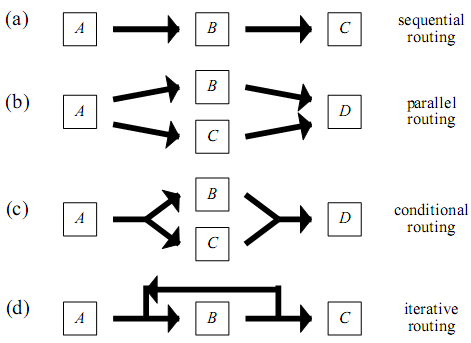
\includegraphics[width=0.7\textwidth]{images/smerovacie_konstrukcie}}
	%popis obrazku
	\caption[smerovacie konštrukcie]{Smerovacie konštrukcie vo workflow systémoch}
	\label{obr:cursus}
\end{figure}


Vo WfMS je možné medzi úlohami použiť smerovacie konštrukcie zobrazené na obrázku :
\begin{itemize}
	\item sekvenčné - úlohy sa vykonávajú za sebou v poradí,v akom nasledujú
	\item paralelné – úlohy sa vykonávajú paralelne nezávisle na sebe za pomoci AND-splitov a AND-joinov.
	\item podmienené – vykonávanie úloh závisí od definovaných podmienok. Realizácia sa vykonáva za pomoci OR-splitov a OR-joinov
	\item iteračné- vykonanie jednej alebo viacerých úloh viackrát za sebou
\end{itemize}

Workflow systémy sú založené na jednotlivých prípadoch (cases). Ako jednotlivý prípad si môžeme predstaviť 	 konkrétnu požiadavku, ako je napríklad založenie si účtu, objednávka, spísanie závete a podobne. Jednotlivé prípady sú častokrát spúšťané samotnými zákazníkmi, ale nie je to pravidlo. Cieľom workflow management systému je efektívne zvládať jednotlivé prípady. Workflow proces je časť workflow management systému zameraný na spracovanie podobných prípadov. Každý workflow proces pozostáva z úloh , ktoré sú za sebou radené v špecifickom poradí. Workflow process definition zabezpečuje , ktorá úloha sa má spustiť a v akom poradí. Veľa prípadov sa môže vykonať s rovnakou postupnosťou. Pri umývaní auta značky Volkswagen postupujeme rovnako ako pri umývaní auta značky Škoda. Jednotlivé úlohy (tasks) sa teda môžu vykonávať súčasne vo viacerých prípadoch. Úloha, ktorá sa vykonáva v konkrétnom prípade, sa nazýva „working item“. Väčšina úloh (working items) je spúšťaná  konkrétnymi zdrojmi. \cite{workflow_systemy}


\subsection{Dopyt po WfMS}
fdsafdsa

\subsection{Výhody použitia WfMS}
fds


\subsection{Riadenie zrojov vo WfMS}
Pod pojmom zdroj rozumieme jednotku, ktorá je určená na vykonávanie úlohy. Môžme si pod tým predstaviť počítač (server, tlačiareň, fax ... ) alebo človeka ako pracovnú jednotku. V business prostredí väčšina zdrojov tvoria jednotliví pracovníci a zákazníci, nie je to však pravidlo.

Jednotlivé zdroje sa môžu zoskupovať do skupín s podobnou charakteristikou. Ak majú rovnakú funkcionálnu charakteristiku, nazývame túto skupinu rola.
Ako príklad role si môžeme predstaviť akúkoľvek pracovnú pozíciu a pod samotnými pracovnými zdrojmi samotného zamestnanca. Táto klasifikácia umožňuje uľahčenie prideľovania právomocí na spúšťanie jednotlivých úloh. Zároveň tak jednotlivé zdroje môžu byť priradené k rôznym roliam a zabráni sa tým problému s nulovou referenciou. Ak by sme priradili jednotlivú úlohu ku konkrétnemu zdroju, nastali by problémy po vymazaní konkrétneho zdroja a samotný proces by nebolo možné ukončiť.


\section{Petriho siete}

//TODO
Definícia \cite{workflow_systemy} :
\begin{quote}
	Petriho sieť orientovaný bipartitný graf s dvoma typmi uzlov nazývaných miesta (places) a prechody (transitions). Uzly sú spojené cez orientované hrany (arcs). Spojenia medzi uzlami rovnakého typu nie sú povolené.
\end{quote}
//TODO



Petriho siete slúžia na matematické modelovanie a simuláciu procesov. Ich hlavná výhoda spočíva v jednoduchosti a grafickej reprezentácii. 


.  V Petriho sieti sa používajú najmä miesta, prechody a tokeny. Miesta určujú stav, v akom sa proces nachádza, prechody slúžia ako prostriedok, ako sa medzi nimi pohybovať. Logiku systému dotvárajú tokeny a hrany. Tokeny určujú, v akom stave sa systém práve nachádza. Podľa typu a násobnosti hrany vieme ,  aké množstvo tokenov je potrebné, aby sa spustil prechod na danú hranu nadväzujúci.


\subsection{Implementovanie Petriho sietí na workflow management systém}
\label{kap:teoria_petriho_siete_na_workflow}

Implementovanie Petriho sietí na workflow management systém je veľmi jednoduché.
Na úrovni procesov sa určuje,  aké úlohy budú za sebou nasledovať a v akom poradí. Modelovanie workflow procesu v Petriho sieti je priamočiare . Úlohy sú reprezentované pomocou prechodou , podmienky sú modelované prostredníctvom  miest a jednotlivé prípady sú zaznačené pomocou tokenov.  Ak chceme Petriho sieť namapovať na workflow systém , musíme zabezpečiť dve konkrétne požiadavky:

a) PN má dve špeciálne miesta: miesto „i“ a miesto „o“, ktoré reprezentujú počiatočný a koncový stav
b) ak pridáme prechod t do PN , ktorý spája miesto „i“ a „o“, potom je PN silno spojená a to znamená, že pre každý pár uzlov x a y  existuje priama cesta od x do y. 

Na obrázku referencia môžeme vidieť jednoduchú implementáciu smerovacích konštrukcii na Petriho sieťach.
Prvá Petriho sieť (a) zobrazuje jednoduché sekvenčné spúšťanie prechodov. V danej sieti  môžeme spúšťať prechody len jednotlivo, v určenom poradí za sebou.
Druhá Petriho sieť (b) predstavuje podmienené spúšťanie úloh. V danej sieti máme na výber z dvoch prechodov, ktoré je možné spustiť.
Tretia Petriho sieť znázorňuje paralelné vykonanie úloh. Po spustení prechodu sa začnú vykonávať dva procesy nezávisle, pričom na konci sa spoja dokopy.
Štvrtá Petriho sieť predstavuje iteračnú konštrukciu, ktorá umožní vrátiť token na predchádzajúci stav.



\section{DAC}


\section{MAC}
\subsection{Model Bell and LaPadula}


\section{RBAC}

\subsection{Popis modelu}

\section{Výhody RBAC}

\subsection{Základné požiadavky}

\subsection{Jadro RBAC}

\subsection{Hierarchické štruktúry}













	


